\documentclass[12pt,a4paper]{article}

% ─── Page Layout ───────────────────────────────────────────────────────────────
\usepackage[a4paper, margin=0.8in, headheight=14pt]{geometry}

% ─── Fonts (XeLaTeX) ───────────────────────────────────────────────────────────
\usepackage{fontspec}
\usepackage{unicode-math}
\setmainfont{TeX Gyre Pagella}
\setmonofont[Scale=0.88]{TeX Gyre Cursor}
\setmathfont{Latin Modern Math}

% ─── Packages ──────────────────────────────────────────────────────────────────
\usepackage{xcolor}
\usepackage{colortbl}
\usepackage{titlesec}
\usepackage{enumitem}
\usepackage{tabularx}
\usepackage{longtable}
\usepackage{booktabs}
\usepackage{array}
\usepackage{amsmath}
\usepackage{tikz}
\usetikzlibrary{shapes.geometric, arrows.meta, positioning, calc, fit, decorations.pathreplacing, patterns}
\usepackage{tcolorbox}
\tcbuselibrary{skins, breakable}
\usepackage{hyperref}
\usepackage{fancyhdr}
\usepackage{graphicx}
\usepackage{microtype}
\hyphenpenalty=10000
\exhyphenpenalty=10000
\sloppy
\usepackage{caption}
\usepackage{setspace}
\usepackage{multirow}
\usepackage{tocloft}

% ─── Q&A helper ────────────────────────────────────────────────────────────────
\newcommand{\Q}[1]{\textbf{#1}\par\noindent\ignorespaces}

% ─── Colour Palette ────────────────────────────────────────────────────────────
\definecolor{myred}{RGB}{196,30,58}
\definecolor{mydark}{RGB}{30,30,50}
\definecolor{mygreen}{RGB}{14,120,80}
\definecolor{myteal}{RGB}{0,130,140}
\definecolor{myamber}{RGB}{180,100,0}
\definecolor{mypurple}{RGB}{100,30,160}
\definecolor{mygray}{RGB}{246,247,249}
\definecolor{mgframe}{RGB}{180,185,200}
\definecolor{watermark}{RGB}{145,150,170}
\definecolor{hdrred}{RGB}{250,232,235}
\definecolor{hdrgreen}{RGB}{220,244,233}
\definecolor{hdrteal}{RGB}{220,242,244}
\definecolor{hdramber}{RGB}{253,242,215}
\definecolor{hdrpurple}{RGB}{238,228,255}
\definecolor{hdrgray}{RGB}{238,240,245}

% ─── Section Formatting ────────────────────────────────────────────────────────
\titleformat{\section}
  {\large\bfseries\color{myred}}{\thesection.}{0.5em}{}
  [\vspace{1pt}{\color{myred}\rule{\linewidth}{0.8pt}}]
\titleformat{\subsection}
  {\normalsize\bfseries\color{myteal}}{\thesubsection}{0.5em}{}
\titlespacing*{\section}{0pt}{18pt}{7pt}
\titlespacing*{\subsection}{0pt}{11pt}{4pt}

% ─── Paragraph ─────────────────────────────────────────────────────────────────
\setlength{\parindent}{0pt}
\setlength{\parskip}{4pt}

% ─── TOC Styling ───────────────────────────────────────────────────────────────
\renewcommand{\cfttoctitlefont}{\large\bfseries\color{myred}}
\renewcommand{\cftaftertoctitle}{\par\noindent{\color{myred}\rule{\linewidth}{0.8pt}}}
\setlength{\cftbeforetoctitleskip}{0pt}
\setlength{\cftaftertoctitleskip}{6pt}
\renewcommand{\cftsecfont}{\normalsize\bfseries\color{mydark}}
\renewcommand{\cftsecpagefont}{\normalsize\bfseries\color{mydark}}
\renewcommand{\cftsecleader}{\cftdotfill{\cftdotsep}}
\setlength{\cftbeforesecskip}{7pt}
\renewcommand{\cftsubsecfont}{\small\color{mydark}}
\renewcommand{\cftsubsecpagefont}{\small\color{mydark}}
\setlength{\cftbeforesubsecskip}{3pt}
\setlength{\cftsubsecindent}{1.4em}

% ─── Table helpers ─────────────────────────────────────────────────────────────
\renewcommand{\arraystretch}{1.45}
\setlength{\tabcolsep}{6pt}
\arrayrulecolor{mydark}
\newcolumntype{B}[1]{>{\small\bfseries\raggedright\arraybackslash}m{#1}}
\newcolumntype{Y}{>{\small\raggedright\arraybackslash}X}
\renewcommand{\tabularxcolumn}[1]{m{#1}}

% ─── Header / Footer ───────────────────────────────────────────────────────────
\pagestyle{fancy}
\fancyhf{}
\fancyhead[L]{\small\color{myred}\textbf{BS-M401}\;\color{mydark}--- Numerical Methods}
\fancyhead[R]{\small\color{myteal}\textbf{Module 1 Notes}}
\fancyfoot[C]{\small\color{mydark}\thepage}
\fancyfoot[R]{\small\color{watermark}\textit{\copyright\ Biraj Sarkar (CGEC)}}
\renewcommand{\headrulewidth}{0.5pt}
\renewcommand{\footrulewidth}{0.3pt}

% ─── Hyperref ──────────────────────────────────────────────────────────────────
\hypersetup{
  colorlinks=true, linkcolor=myteal, urlcolor=myteal,
  pdfauthor={Biraj Sarkar (CGEC)},
  pdftitle={BS-M401 --- Module 1 Notes: Numerical Errors, Interpolation and Integration}
}

% ─── tcolorbox styles ──────────────────────────────────────────────────────────
\tcbset{
  tikzbox/.style={
    colback=mygray, colframe=mgframe, boxrule=0.6pt, arc=4pt,
    left=8pt, right=8pt, top=6pt, bottom=6pt,
    colbacktitle=mgframe, coltitle=mydark, fonttitle=\small\bfseries
  },
  defbox/.style={
    colback=hdrgreen, colframe=mygreen, boxrule=0.8pt, arc=4pt,
    left=9pt, right=9pt, top=6pt, bottom=6pt,
    colbacktitle=mygreen, coltitle=white, fonttitle=\small\bfseries
  },
  formulabox/.style={
    colback=hdrteal, colframe=myteal, boxrule=0.8pt, arc=4pt,
    left=9pt, right=9pt, top=7pt, bottom=7pt,
    colbacktitle=myteal, coltitle=white, fonttitle=\small\bfseries
  },
  examplebox/.style={
    colback=hdramber, colframe=myamber, boxrule=0.8pt, arc=4pt,
    left=9pt, right=9pt, top=6pt, bottom=6pt,
    colbacktitle=myamber, coltitle=white, fonttitle=\small\bfseries
  },
  masonbox/.style={
    colback=hdrpurple, colframe=mypurple, boxrule=0.8pt, arc=4pt,
    left=9pt, right=9pt, top=6pt, bottom=6pt,
    colbacktitle=mypurple, coltitle=white, fonttitle=\small\bfseries
  },
  exambox/.style={
    colback=hdrpurple, colframe=mypurple, boxrule=1pt, arc=5pt,
    left=10pt, right=10pt, top=8pt, bottom=8pt,
    colbacktitle=mypurple, coltitle=white, fonttitle=\bfseries,
    breakable, title after break={\textbf{Frequently Asked / Viva Questions (contd.)}}
  }
}
\tcbset{breakable}
\tcbset{after={\par\color{black}}}

% ─── TikZ styles ───────────────────────────────────────────────────────────────
\tikzset{
  block/.style={rectangle, draw=myteal, fill=hdrteal,
    text width=2.4cm, align=center, minimum height=0.95cm,
    font=\small, rounded corners=3pt, line width=0.7pt},
  redblock/.style={rectangle, draw=myred, fill=hdrred,
    text width=2.4cm, align=center, minimum height=0.95cm,
    font=\small, rounded corners=3pt, line width=0.7pt},
  amberblock/.style={rectangle, draw=myamber, fill=hdramber,
    text width=2.4cm, align=center, minimum height=0.95cm,
    font=\small, rounded corners=3pt, line width=0.7pt},
  sumjunc/.style={circle, draw=myamber, fill=hdramber,
    minimum size=0.62cm, font=\small, line width=0.8pt},
  arrow/.style={-Stealth, thick, color=mydark},
  redarrow/.style={-Stealth, thick, color=myred},
  line/.style={thick, color=mydark}
}

\begin{document}

% ─── Title Page ───────────────────────────────────────────────────────────────
\begin{center}
  {\LARGE\bfseries\color{myred} BS-M401 --- Numerical Methods}\\[5pt]
  {\normalsize\color{mydark} Semester IV \quad$\bullet$\quad 2L:0T:0P \quad$\bullet$\quad 2 Credits}\\[3pt]
  {\normalsize\color{myteal}\textbf{Module 1 Exam Notes: Numerical Errors, Interpolation and Integration}}\\[3pt]
  {\small\color{mydark} CGEC \;$|$\; B.Tech ECE (2023--27) \;$|$\; \textit{Biraj Sarkar}}
\end{center}
\vspace{2pt}
\noindent{\color{myred}\rule{\linewidth}{1.5pt}}
\vspace{2pt}

\hypersetup{linkcolor=mydark}
\tableofcontents
\hypersetup{linkcolor=myteal}
\newpage

\section{Numerical Errors, Interpolation and Integration}
\subsection{Approximation and types of error}
\begin{tcolorbox}[defbox, title={Numerical approximation}]
A numerical method replaces an exact mathematical operation by a finite computation. If $x$ is the true value and $\hat{x}$ its approximation, use the signed-error convention $e=x-\hat{x}$. The absolute error is $|e|$.
\end{tcolorbox}

\begin{itemize}[leftmargin=*, itemsep=3pt, topsep=4pt]
  \item \textbf{Relative error.} Use $|e|/|x|$ for $x\ne0$. Multiply by $100$ for percentage error. For an exact value of zero, report absolute error.
  \item \textbf{Truncation error.} This comes from cutting short an infinite process or replacing a continuous operation by a finite formula.
  \item \textbf{Round-off error.} This comes from storing or carrying out arithmetic with finitely many digits. Round-off may accumulate when operations are repeated.
  \item \textbf{Input error.} A computation can also inherit measurement error already present in its data. A finer mesh does not make the original measurements more accurate.
\end{itemize}
\begin{tcolorbox}[examplebox, title={Separate the two error sources}]
Use the first three terms of the exponential series at $x=0.1$.
\[
\begin{aligned}
1+x+\frac{x^2}{2}&=1.105,\\
e^{0.1}-1.105&\approx0.000170186.
\end{aligned}
\]
The second line is truncation error. If the computed $1.105$ is then rounded to two decimal places with ties rounded upward, the stored value is $1.11$. The additional signed round-off error is $1.105-1.11=-0.005$. The total signed error is the sum, about $-0.004829814$.
\end{tcolorbox}

\subsection{Fixed-point and floating-point arithmetic}
\par\vspace{5pt}
\begingroup
\setlength{\extrarowheight}{1pt}
\noindent\begin{tabularx}{\linewidth}{|B{3.1cm}|Y|Y|}
\hline
\textbf{Representation} & \textbf{How numbers are stored} & \textbf{Practical consequence} \\ \hline
Fixed point & Store an integer $N$ with a fixed scale, such as $N/10^2$ or $N/2^f$. & Uniform spacing. With $f$ binary fractional bits the spacing is $2^{-f}$. Range depends on integer width. \\ \hline
Floating point & Store sign, significand and exponent. A normalized decimal model has form $\pm d.dd\ldots\times10^e$. & Spacing increases with magnitude. Finite precision and exponent limits give round-off, overflow and underflow. \\ \hline
\end{tabularx}\par
\endgroup
\begin{enumerate}[leftmargin=*, itemsep=3pt, topsep=4pt]
  \item \textbf{Fixed-point example.} At scale $10^{-2}$, store $12.34$ as $1234$ and $0.57$ as $57$. Add the integers to get $1291$, representing $12.91$. For multiplication, the raw product has scale $10^{-4}$ and must be rescaled before storing.
  \item \textbf{Floating-point addition.} Align exponents, add significands, normalize the result, then round. At four significant digits, $1.234\times10^3+5.678\times10^{-2}$ rounds to $1.234\times10^3$. The smaller addend is lost at this precision.
  \item \textbf{Floating-point multiplication.} Multiply the significands, add exponents, then normalize and round. This is different from addition, where exponents are aligned.
\end{enumerate}
For $p$ significant digits in base $\beta$, round-to-nearest gives a relative rounding bound $u=\tfrac12\beta^{1-p}$ for normal results in range. For an exact result $z$ away from overflow and underflow, write $\mathrm{fl}(z)=z(1+\delta)$ with $|\delta|\le u$.
\begin{tcolorbox}[masonbox, title={Cancellation}]
Subtracting nearly equal approximations can leave very few correct digits. At four significant digits, $\sqrt{10001}$ rounds to $100.0$, so the direct difference $\sqrt{10001}-100$ becomes zero. Rationalise it as $1/(\sqrt{10001}+100)$ to obtain approximately $0.005000$. The exact expression is the same, but the evaluation avoids the harmful subtraction.
\end{tcolorbox}

\subsection{Propagation of errors}
\begin{tcolorbox}[formulabox, title={First-order propagation}]
Let the inputs be perturbed by $\Delta x_i=\hat x_i-x_i$. For differentiable $g$,
\[
\Delta g \approx \sum_{i=1}^n
  \frac{\partial g}{\partial x_i}\Delta x_i,\qquad
|\Delta g|\lesssim\sum_{i=1}^n
  \left|\frac{\partial g}{\partial x_i}\right|\,|\Delta x_i|.
\]
This is a first-order estimate. State the evaluation point and use it for sufficiently small perturbations.
\end{tcolorbox}

\begin{itemize}[leftmargin=*, itemsep=3pt, topsep=4pt]
  \item \textbf{Sum or difference.} Absolute error is bounded by the sum of the absolute input errors. Relative error can still be large when the exact result is close to zero.
  \item \textbf{Product.} $(x+\Delta x)(y+\Delta y)-xy=y\Delta x+x\Delta y+\Delta x\Delta y$. Divide by $xy$ and neglect the product of relative errors for a first-order estimate.
  \item \textbf{Quotient.} For $x,y\ne0$, the first-order relative change is $\Delta x/x-\Delta y/y$. If the denominator could approach zero, the quotient can be very sensitive.
\end{itemize}
\begin{tcolorbox}[examplebox, title={Propagate measurement errors in an area}]
Let $A=lb$, where $l=10.00\pm0.02$ cm and $b=5.00\pm0.01$ cm. The nominal area is $50.00\ \mathrm{cm}^2$. The first-order absolute error estimate is
\[
\begin{aligned}
|\Delta A|&\lesssim b|\Delta l|+l|\Delta b|\\
           &=5(0.02)+10(0.01)
            =0.20\ \mathrm{cm}^2.
\end{aligned}
\]
The neglected product term has magnitude at most $0.0002\ \mathrm{cm}^2$. The first-order relative error is about $0.4\%$.
\end{tcolorbox}

\section{Polynomial Interpolation}
\subsection{Choosing a method and estimating the remainder}
\begin{tcolorbox}[defbox, title={Interpolation}]
Interpolation estimates an unknown value inside a range of known data points. At $n+1$ distinct nodes, there is a unique polynomial $P_n$ of degree at most $n$ passing through all the samples. Evaluating it outside that range is extrapolation.
\end{tcolorbox}

\begin{itemize}[leftmargin=*, itemsep=3pt, topsep=4pt]
  \item \textbf{Equal spacing near the beginning.} Newton forward differences keep the normalized offset small.
  \item \textbf{Equal spacing near the end.} Newton backward differences use the last point as reference.
  \item \textbf{Unequal spacing.} Use Lagrange or Newton divided differences. These also work for equally spaced nodes.
\end{itemize}
\begin{tcolorbox}[formulabox, title={Interpolation remainder}]
If $f$ has $n+1$ continuous derivatives on an interval containing the nodes and evaluation point, then for a suitable $\xi$ in that interval,
\[
f(x)-P_n(x)=
 \frac{f^{(n+1)}(\xi)}{(n+1)!}
 \prod_{j=0}^{n}(x-x_j).
\]
The error is zero at a node. Bound the derivative and the product separately for an error estimate.
\end{tcolorbox}

\subsection{Newton forward and backward differences}
For equally spaced nodes $x_i=x_0+ih$, define $\Delta y_i=y_{i+1}-y_i$ and $\nabla y_i=y_i-y_{i-1}$. Higher differences repeat the same operation.
\begin{tcolorbox}[formulabox, title={Forward and backward formulas}]
\[
\begin{aligned}
P_n(x)&=y_0+u\Delta y_0
       +\frac{u(u-1)}{2!}\Delta^2y_0+\cdots,
       &&u=\frac{x-x_0}{h},\\
P_n(x)&=y_n+v\nabla y_n
       +\frac{v(v+1)}{2!}\nabla^2y_n+\cdots,
       &&v=\frac{x-x_n}{h}.
\end{aligned}
\]
The order-$k$ forward coefficient uses factors $u,u-1,\ldots,u-k+1$. The backward coefficient uses $v,v+1,\ldots,v+k-1$. Divide each product by $k!$.
\end{tcolorbox}

\begin{tcolorbox}[examplebox, title={Build one difference table and use both ends}]
For the samples of $f(x)=x^3+x$ at step $h=1$:
\par\vspace{5pt}
\begingroup
\setlength{\extrarowheight}{1pt}
\noindent\begin{tabularx}{\linewidth}{|B{1.65cm}|Y|Y|Y|Y|}
\hline
\textbf{$x$} & \textbf{$y$} & \textbf{$Delta y$} & \textbf{$Delta^2 y$} & \textbf{$Delta^3 y$} \\ \hline
$0$ & $0$ & $2$ & $6$ & $6$ \\ \hline
$1$ & $2$ & $8$ & $12$ &  \\ \hline
$2$ & $10$ & $20$ &  &  \\ \hline
$3$ & $30$ &  &  &  \\ \hline
\end{tabularx}\par
\endgroup
The head of the table gives forward differences $2,6,6$. For $x=0.5$, $u=0.5$:
\[
\begin{aligned}
P_3(0.5)&=0+(0.5)(2)
  +\frac{(0.5)(-0.5)}{2}(6)
  +\frac{(0.5)(-0.5)(-1.5)}{6}(6)\\
 &=0.625.
\end{aligned}
\]
At the other end, $\nabla y_3=20$, $\nabla^2y_3=12$, and $\nabla^3y_3=6$. For $x=2.5$, $v=-0.5$:
\[
\begin{aligned}
P_3(2.5)&=30+(-0.5)(20)
 +\frac{(-0.5)(0.5)}{2}(12)
 +\frac{(-0.5)(0.5)(1.5)}{6}(6)\\
 &=18.125.
\end{aligned}
\]
\end{tcolorbox}

\subsection{Lagrange and Newton divided differences}
\begin{tcolorbox}[formulabox, title={Lagrange basis and Newton coefficients}]
\[
\begin{aligned}
P_n(x)&=\sum_{i=0}^n y_i L_i(x),
& L_i(x)&=\prod_{\substack{0\le j\le n\\j\ne i}}
 \frac{x-x_j}{x_i-x_j},\\
f[x_i,\ldots,x_{i+k}] &=
\frac{f[x_{i+1},\ldots,x_{i+k}]-f[x_i,\ldots,x_{i+k-1}]}
{x_{i+k}-x_i}. &&
\end{aligned}
\]
The divided-difference base is $f[x_i]=y_i$. The coefficient of $\prod_{j=0}^{k-1}(x-x_j)$ is $f[x_0,\ldots,x_k]$ in Newton form. Each term obeys the previously fitted data because its extra factor vanishes at the earlier nodes.
\end{tcolorbox}

\begin{tcolorbox}[examplebox, title={Unequal nodes: find the same value by two methods}]
Use $(0,1),(1,3),(3,13)$. At $x=2$ the Lagrange basis values are $-1/3$, $1$, and $1/3$, respectively, so $P_2(2)=-1/3+3+13/3=7$.

\textbf{Newton table.} The first divided differences are $(3-1)/(1-0)=2$ and $(13-3)/(3-1)=5$. The second divided difference is $(5-2)/(3-0)=1$. Hence
\[
P_2(x)=1+2(x-0)+(x-0)(x-1),\qquad P_2(2)=7.
\]
Adding a new distinct node in Newton form adds a new product term without changing earlier coefficients.
\end{tcolorbox}

\begin{tcolorbox}[masonbox, title={Difference table check}]
For equally spaced nodes, $f[x_0,\ldots,x_k]=\Delta^k y_0/(k!h^k)$. The factors $h$ cancel when Newton divided differences are written in terms of $u$. This gives the Newton forward formula.
\end{tcolorbox}

\section{Numerical Integration}
\subsection{Trapezoidal rule}
\begin{tcolorbox}[defbox, title={Quadrature and panel width}]
Quadrature approximates an integral by a weighted sum of function values. For $N$ equal subintervals from $a$ to $b$, use $h=(b-a)/N$, $x_i=a+ih$ and $y_i=f(x_i)$. Write errors as exact integral minus approximation.
\end{tcolorbox}

\begin{tcolorbox}[formulabox, title={Trapezoidal rule and error}]
Integrating the straight interpolant through the two endpoints of a panel of width $h$ gives $h(y_i+y_{i+1})/2$. Interior endpoints occur twice when panels are added:
\[
T_N=h\left[\frac{y_0+y_N}{2}+\sum_{i=1}^{N-1}y_i\right].
\]
The one-panel error is $-h^3 f''(\xi)/12$. The composite error is $I-T_N=-(b-a)h^2 f''(\xi)/12$ for continuous $f''$. To see the local constant, integrate the interpolation remainder $\tfrac12 f''(\xi_x)(x-x_i)(x-x_{i+1})$. The quadratic factor keeps one sign on the panel, so $\tfrac12\int_0^h t(t-h)\,dt=-h^3/12$ is the coefficient at some point $\xi$.
\end{tcolorbox}

\begin{tcolorbox}[tikzbox, title={Trapezoidal approximation on one panel}]
\centering
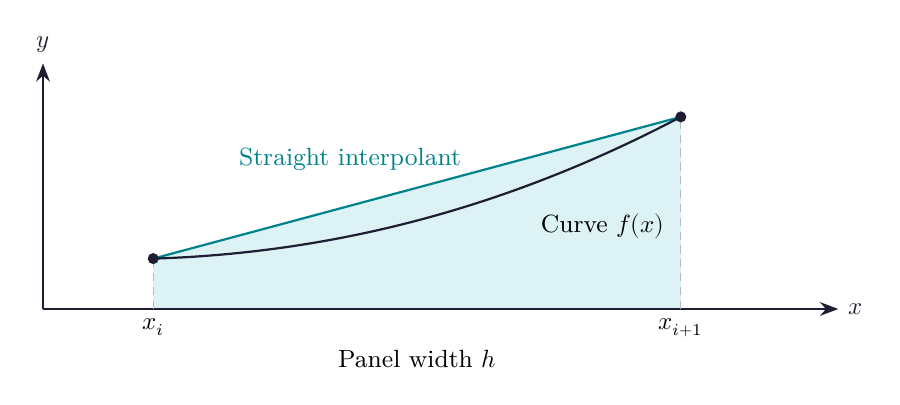
\begin{tikzpicture}[y=0.80cm,every node/.style={font=\small}]
  \fill[hdrteal] (1.4,0)--(8.1,0)--(8.1,3.05)--(1.4,0.8)--cycle;
  \draw[arrow] (0,0)--(10.1,0) node[right] {$x$};
  \draw[arrow] (0,0)--(0,3.9) node[above] {$y$};
  \draw[myteal,thick] (1.4,0.8)--(8.1,3.05);
  \draw[mydark,thick] (1.4,0.8) .. controls (4,0.9) and (6.2,1.8) .. (8.1,3.05);
  \draw[mgframe,densely dashed] (1.4,0)--(1.4,0.8) (8.1,0)--(8.1,3.05);
  \fill[mydark] (1.4,0.8) circle (2pt) (8.1,3.05) circle (2pt);
  \node[below] at (1.4,0) {$x_i$};
  \node[below] at (8.1,0) {$x_{i+1}$};
  \node[below] at (4.75,-0.5) {Panel width $h$};
  \node[above,text=myteal] at (3.9,2.04) {Straight interpolant};
  \node[right] at (6.2,1.32) {Curve $f(x)$};
\end{tikzpicture}\par
\end{tcolorbox}

\subsection{Simpson's one-third rule}
\begin{tcolorbox}[formulabox, title={Simpson weights and error}]
Use an even number $N$ of equal subintervals. On one two-subinterval panel, integrate the quadratic interpolant through $m-h,m,m+h$. Its three basis integrals are $h/3,4h/3,h/3$.
\[
S_N=\frac{h}{3}\left[y_0+y_N
    +4\!\!\!\sum_{\substack{1\le i<N\\ i\ \mathrm{odd}}}\!y_i
    +2\!\!\!\sum_{\substack{2\le i<N\\ i\ \mathrm{even}}}\!y_i\right].
\]
The panel error is $-h^5 f^{(4)}(\xi)/90$. The composite error is $I-S_N=-(b-a)h^4f^{(4)}(\xi)/180$ for continuous $f^{(4)}$. Here $h$ is one subinterval, so a single panel has width $2h$.
\end{tcolorbox}

\begin{enumerate}[leftmargin=*, itemsep=3pt, topsep=4pt]
  \item \textbf{Why the rule is exact through degree three.} It integrates the quadratic interpolant exactly. A cubic's remaining odd part about the midpoint contributes zero to both the integral and the symmetric weighted sum.
  \item \textbf{Where the error constant comes from.} Use the cubic Hermite interpolant that matches the three sampled values and the midpoint derivative. Its error factor, with $t=x-m$, is $(t+h)t^2(t-h)$. It has one sign across the panel.
  \item \textbf{Integrate the factor.} The Hermite remainder multiplies that factor by $f^{(4)}(\xi_x)/4!$. Integrating the factor gives $-4h^5/15$. Division by $4!$ yields $-h^5/90$, and summing $(b-a)/(2h)$ panels gives the composite constant.
\end{enumerate}
\begin{tcolorbox}[examplebox, title={Compare rules and their signed errors on the same data}]
Integrate $x^4$ from $0$ to $2$. Use $N=2$ and $h=1$, giving ordinates $0,1,16$.
\[
\begin{aligned}
I&=\frac{2^5}{5}=\frac{32}{5},\\
T_2&=\frac{0+16}{2}+1=9,\\
S_2&=\frac{0+4(1)+16}{3}=\frac{20}{3}.
\end{aligned}
\]
The signed errors are $I-T_2=-13/5$ and $I-S_2=-4/15$. With $f^{(4)}=24$, Simpson's formula agrees: $-2(24)/180=-4/15$.
\end{tcolorbox}

\newpage
\begin{center}
  {\large\bfseries\color{myred} Quick Revision --- Module 1}\\[3pt]
  {\small\color{mydark} Numerical Errors, Interpolation and Integration $|$ BS-M401}
\end{center}
\noindent{\color{myred}\rule{\linewidth}{1.2pt}}\par\vspace{4pt}

\begin{tcolorbox}[formulabox, title={Key Concepts at a Glance}]
\renewcommand{\arraystretch}{1.35}
\noindent\begin{tabularx}{\linewidth}{B{4.5cm}Y}
Signed error & $e=x-\hat x$. Relative error is $|e|/|x|$ when $x\ne0$. \\[3pt]
Error propagation & $\Delta g\approx\sum_i(\partial g/\partial x_i)\Delta x_i$. \\[3pt]
Newton offsets & $u=(x-x_0)/h$ for forward and $v=(x-x_n)/h$ for backward. \\[3pt]
Quadrature errors & Composite trapezoidal error is order $h^2$. Composite Simpson error is order $h^4$ under smoothness assumptions. \\[3pt]
\end{tabularx}\par
\end{tcolorbox}

\begin{tcolorbox}[defbox, title={One-Line Definitions}]
\begin{itemize}[leftmargin=*, itemsep=3pt, topsep=4pt]
  \item \textbf{Round-off.} Error introduced by finite digit storage or arithmetic.
  \item \textbf{Truncation.} Error introduced by replacing an exact procedure by a finite approximation.
  \item \textbf{Interpolation.} Estimate inside the sampled range.
  \item \textbf{Quadrature.} Approximate an integral using sampled function values.
\end{itemize}
\end{tcolorbox}

\begin{tcolorbox}[exambox, title={Frequently Asked / Viva Questions}]
\begin{enumerate}[topsep=0pt, label=\textbf{Q\arabic*.}, itemsep=5pt, leftmargin=*]
  \item \Q{Why can subtraction lose significant digits?}
    Errors in similar operands can dominate their small difference.
  \item \Q{What is the spacing with $f$ fixed binary fractional bits?}
    $2^{-f}$.
  \item \Q{What happens first in floating-point addition?}
    Align both significands to the same exponent.
  \item \Q{How does the first-order product error combine?}
    The signed relative changes add to first order.
  \item \Q{When is Newton forward preferred?}
    Nodes are equally spaced and the target is near the beginning.
  \item \Q{What changes in the Newton backward coefficients?}
    Use rising products in $v=(x-x_n)/h$ and differences at the last node.
  \item \Q{What is the advantage of Newton divided differences?}
    Unequal nodes are allowed, and another node adds a term to the existing polynomial.
  \item \Q{What is $L_i(x_j)$?}
    It is one if $i=j$ and zero otherwise.
  \item \Q{What subinterval count does composite Simpson require?}
    An even count of equal subintervals.
  \item \Q{What are the trapezoidal and Simpson degrees of exactness?}
    One and three, respectively.
  \item \Q{How does halving the step affect smooth composite error bounds?}
    The trapezoidal bound falls by a factor of four and the Simpson bound by sixteen under the same derivative bounds.
\end{enumerate}
\end{tcolorbox}

\begin{tcolorbox}[tikzbox, title={Summary Comparison}]
\par\vspace{5pt}
\begingroup
\setlength{\extrarowheight}{1pt}
\noindent\begin{tabularx}{\linewidth}{|B{3.45cm}|Y|Y|}
\hline
\textbf{Method} & \textbf{Where to apply} & \textbf{Check before using} \\ \hline
Newton forward or backward & Uniform nodes, near one end. & Choose the right end and maintain the sign of the offset. \\ \hline
Lagrange or divided differences & Any distinct nodes. & Keep the indices and node spacings in order. \\ \hline
Trapezoidal & Uniform composite grid for the stated formula. & Half-weight the endpoints. \\ \hline
Simpson one-third & Uniform grid with even subinterval count. & Use alternating weights 4 and 2 on the interior. \\ \hline
\end{tabularx}\par
\endgroup
\end{tcolorbox}

\end{document}
